% Lecture 7 slides (sem1). Canvases: statements and figures; proofs are written live.
\documentclass{ca-slides}

\lecture{7}{Порядок элемента и первообразные корни}
\author{}

\begin{document}
\titleframe

\begin{canvasframe}{Зачем нужны порядки}
  \small
  \begin{itemize}
    \item Общие параметры: простое $p$ и $g \in \Znx{p}$; ключ $K = g^{ab}$
    \item Полиг"--~Хеллман (2-й семестр): DLP решается за $\approx \sqrt{q}$, где $q$ "---
      наибольший простой делитель $\ord g$
    \item Нужно уметь:
    \begin{itemize}
      \item вычислять $\ord g$;
      \item находить образующий $\Znx{p}$ (первообразный корень) или элемент большого
        простого порядка;
      \item понимать, когда $\Znx{n}$ циклическая
    \end{itemize}
    \item Всё это "--- \textbf{при известном разложении} $\abs{G}$
  \end{itemize}
\end{canvasframe}

\begin{canvasframe}{Группы и порядки элементов}
  \small
  \begin{definition}
    $\ord g$ "--- наименьшее $m \ge 1$ с $g^m = 1$;\quad
    $\langle g \rangle = \{g^k\}$;\quad $G$ \emph{циклическая}, если $G = \langle g \rangle$
    ($g$ "--- \emph{образующий}).
  \end{definition}
  \begin{proposition}
    Если $\ord g = m$, то $g^k = 1 \iff m \mid k$, и $\abs{\langle g \rangle} = m$.
  \end{proposition}
  Примеры: $\Zn{n}$, $\Znx{n}$ (порядок $\varphi(n)$), $\GF{q}^*$, точки кривой.
  \aside{почему в конечной группе порядок конечен?}
\end{canvasframe}

\begin{theoremframe}[theorem]{Теорема Лагранжа}
  Если $H \le G$, $G$ конечна, то $\abs{H} \mid \abs{G}$.

  \smallskip
  \textbf{Следствие.} $\ord g \mid \abs{G}$, $g^{\abs{G}} = 1$; теоремы Эйлера и Ферма.
\end{theoremframe}

\begin{theoremframe}[theorem]{Порядок степени}
  Если $\ord g = m$, то \[\ord\bigl(g^k\bigr) = \frac{m}{\gcd(k, m)}.\]
  \textbf{Следствие.} В циклической группе порядка $n$: образующих $\varphi(n)$; элементов
  порядка $d \mid n$ ровно $\varphi(d)$; $\sum_{d \mid n} \varphi(d) = n$.
\end{theoremframe}

\begin{canvasframe}{Критерий порядка}
  \begin{lemma}
    $\ord g = m \iff g^m = 1$ и $g^{m/q} \ne 1$ для каждого простого $q \mid m$.
  \end{lemma}
  \begin{lemma}
    Абелева группа, $\ord a = r$, $\ord b = s$, $\gcd(r, s) = 1$ $\Rightarrow$ $\ord(ab) = rs$.
  \end{lemma}
  \aside{пример в $\Znx{8}$, где взаимная простота нарушена}
\end{canvasframe}

\begin{canvasframe}{Вычисление порядка}
  \begin{itemize}
    \item Дано: $g \in G$ и $N = \abs{G} = q_1^{e_1} \cdots q_r^{e_r}$ (или любое кратное
      $\ord g$) \textbf{с разложением}
    \item $\omega(N) = r$, $\Omega(N) = e_1 + \cdots + e_r \le \log_2 N$,
      $\omega(N) = \bigO(\log N / \log\log N)$
    \item Перебор делителей: до $\tau(N)$ возведений в степень "--- слишком много
    \item Идея: идти \emph{сверху}, от $N$, убирая простые множители
  \end{itemize}
  \aside{сколько делителей у $N = 2 \cdot 3 \cdot 5 \cdots 29$?}
  \penspace[0.25\textheight]
\end{canvasframe}

\begin{canvasframe}{Последовательное снижение}
  \small
  \begin{algorithm}
  \begin{algorithmic}[1]
    \State $o \gets N$
    \For{$i = 1, \dots, r$}
      \For{$j = 1, \dots, e_i$}
        \If{$g^{o/q_i} \ne 1$} \textbf{перейти} к следующему $i$ \EndIf
        \State $o \gets o / q_i$
      \EndFor
    \EndFor
    \State \Return $o$
  \end{algorithmic}
  \end{algorithm}
  \begin{theorem}
    Результат "--- $\ord g$; $\le \Omega(N)$ возведений, $\bigO(\log^2 N)$ операций.
  \end{theorem}
\end{canvasframe}

\begin{canvasframe}{Пример: $p = 61$, $g = 13$}
  $N = 60 = 2^2 \cdot 3 \cdot 5$
  \[
  \begin{array}{llll}
    q = 2: & 13^{30} \equiv 1, & o \gets 30; & 13^{15} \equiv 1, \ o \gets 15\\
    q = 3: & 13^{5} \equiv 47 \ne 1, & o = 15; & \\
    q = 5: & 13^{3} \equiv 1, & o \gets 3. &
  \end{array}
  \]
  $\ord 13 = 3$.
  \penspace[0.35\textheight]
\end{canvasframe}

\begin{canvasframe}{Разделение по делителям}
  \begin{lemma}
    $m = \ord g \mid N$, $h_i = g^{N/q_i^{e_i}}$ $\Rightarrow$ $\ord h_i = q_i^{v_{q_i}(m)}$,\quad
    $\ord g = \prod_i \ord h_i$.
  \end{lemma}
  \begin{itemize}
    \item $\ord h_i$: $h_i \to h_i^{q_i} \to h_i^{q_i^2} \to \dots \to 1$; в сумме
      $\bigO(\log N)$ операций
    \item Все $h_i$ по отдельности: $\omega(N)$ возведений, $\bigO(\omega(N) \log N)$
    \item Можно ли \emph{совместно}?
  \end{itemize}
\end{canvasframe}

\begin{canvasframe}{Дерево произведений}
  \centering
  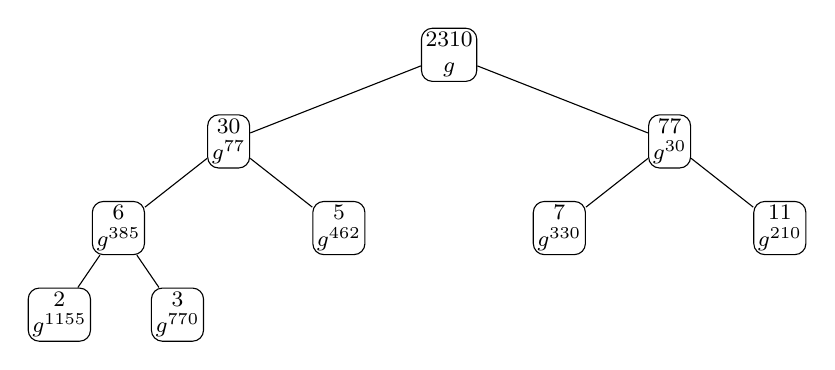
\begin{tikzpicture}[
      level distance=11mm,
      level 1/.style={sibling distance=56mm},
      level 2/.style={sibling distance=28mm},
      level 3/.style={sibling distance=15mm},
      every node/.style={draw, rounded corners, inner sep=1.5pt, font=\footnotesize, align=center}]
    \node {$2310$\\ $g$}
      child { node {$30$\\ $g^{77}$}
        child { node {$6$\\ $g^{385}$}
          child { node {$2$\\ $g^{1155}$} }
          child { node {$3$\\ $g^{770}$} } }
        child { node {$5$\\ $g^{462}$} } }
      child { node {$77$\\ $g^{30}$}
        child { node {$7$\\ $g^{330}$} }
        child { node {$11$\\ $g^{210}$} } };
  \end{tikzpicture}

  \raggedright\small
  Инвариант: узлу $S$ соответствует $h_S = g^{N/P_S}$;\quad
  $h_L = h_S^{P_R}$, \ $h_R = h_S^{P_L}$ \ \textcolor{caRed}{\textbf{?}~\itshape почему?}
\end{canvasframe}

\begin{canvasframe}{Дерево произведений: алгоритм}
  \begin{algorithm}
  \begin{algorithmic}[1]
    \Function{Down}{$S$, $h$} \Comment{$h = g^{N/P_S}$}
      \If{$S = \{i\}$} $h_i \gets h$; \Return \EndIf
      \State $S = L \sqcup R$:\ \Call{Down}{$L$, $h^{P_R}$};\ \Call{Down}{$R$, $h^{P_L}$}
    \EndFunction
    \State \Call{Down}{$\{1..r\}$, $g$}; \ $k_i$: число шагов $h_i \gets h_i^{q_i}$ до $1$
    \State \Return $\prod_i q_i^{k_i}$
  \end{algorithmic}
  \end{algorithm}
  \begin{theorem}
    $\bigO(\log N \cdot \log \omega(N)) = \bigO(\log N \log\log N)$ групповых операций.
  \end{theorem}
\end{canvasframe}

\begin{canvasframe}{Пример: $p = 421$, $g = 37$}
  $N = 420 = 2^2 \cdot 3 \cdot 5 \cdot 7$; дерево: $420$; \ $12,\ 35$; \ $4,\ 3,\ 5,\ 7$
  \begin{itemize}
    \item корень: $h = 37$: \ $h^{35} \equiv 392$, \ $h^{12} \equiv 49$
    \item узел $\{4, 3\}$, $h = 392$: \ $h^{3} \equiv 29$, \ $h^{4} \equiv 1$
    \item узел $\{5, 7\}$, $h = 49$: \ $h^{7} \equiv 279$, \ $h^{5} \equiv 247$
    \item листья: $4$: $29 \to 420 \to 1$; \ $3$: $1$; \ $5$: $279 \to 1$; \ $7$: $247 \to 1$
  \end{itemize}
  \[\ord 37 = 2^2 \cdot 3^0 \cdot 5 \cdot 7 = 140\]
  \penspace[0.1\textheight]
\end{canvasframe}

\begin{canvasframe}{Многочлены над полем}
  \begin{lemma}
    Ненулевой многочлен степени $d$ над полем $K$ имеет не более $d$ корней в $K$.
  \end{lemma}
  \proofarea[0.25\textheight]
  \aside{сколько корней у $x^2 - 1$ в $\Zn{8}$?}
\end{canvasframe}

\begin{theoremframe}[theorem]{Цикличность $\Znx{p}$}
  Конечная подгруппа мультипликативной группы поля циклическая. В частности, $\Znx{p}$ и
  $\GF{q}^*$ циклические.

  \smallskip
  \textbf{Следствие.} По модулю $p$ ровно $\varphi(p - 1)$ первообразных корней:
  $g^k$, $\gcd(k, p - 1) = 1$.
\end{theoremframe}

\begin{canvasframe}{Критерий корня}
  \begin{theorem}
    Пусть $\gcd(g, n) = 1$, $q_1, \dots, q_r$ "--- простые делители $\varphi(n)$. Тогда $g$ "---
    первообразный корень по модулю $n$ $\iff$ $g^{\varphi(n)/q_i} \not\equiv 1 \pmod n$ для
    всех $i$.
  \end{theorem}
  \begin{itemize}
    \item Стоимость проверки: $\omega(\varphi(n))$ возведений в степень
    \item Поиск наименьшего: $g = 2, 3, \dots$; пропускаем квадраты и $\gcd(g, n) > 1$
  \end{itemize}
  \aside{почему квадрат $h^2$ не может быть первообразным корнем?}
  \penspace[0.15\textheight]
\end{canvasframe}

\begin{canvasframe}{Пример: $p = 41$}
  $p - 1 = 40 = 2^3 \cdot 5$; показатели $20$ и $8$:
  \[
  \begin{array}{c|cc|l}
    g & g^{20} & g^{8} & \\ \hline
    2 & 1 & & \text{нет} \\
    3 & 40 & 1 & \text{нет} \\
    4 & & & = 2^2 \\
    5 & 1 & & \text{нет} \\
    6 & 40 & 10 & \text{корень}
  \end{array}
  \]
  Всего первообразных корней: $\varphi(40) = 16$.
  \penspace[0.15\textheight]
\end{canvasframe}

\begin{canvasframe}{Стоимость поиска}
  \begin{itemize}
    \item Доля корней: $\dfrac{\varphi(p-1)}{p-1} = \prod_{q \mid p-1}\Bigl(1 - \dfrac1q\Bigr)
      \ge \dfrac{c}{\ln\ln p}$
    \item Эвристически $\bigO(\log\log p)$ кандидатов, всего
      $\bigO(\log\log p \cdot \omega(p - 1) \cdot \log p)$ умножений
    \item На практике $g$ мало: для $p < 10^4$ \ $g \le 31$; $2$ "--- корень для $\approx 37{,}4\,\%$
      простых (гипотеза Артина)
    \item Узкое место "--- \textbf{разложение $p - 1$}
  \end{itemize}
  \penspace[0.2\textheight]
\end{canvasframe}

\begin{theoremframe}[proposition]{Безопасные простые}
  Для $2 \le g \le p - 2$: \ $g$ "--- первообразный корень $\iff g^q \equiv -1 \pmod p$;
  иначе $\ord g = q$.

  \smallskip
  Пример: $p = 23$: \ $2^{11} \equiv 3^{11} \equiv 1$, \ $5^{11} \equiv -1$ $\Rightarrow$ $g = 5$.
\end{theoremframe}

\begin{canvasframe}{Составной модуль}
  \begin{theorem}[Гаусс]
    Первообразные корни по модулю $n$ существуют $\iff$
    \[n \in \{1, 2, 4, p^k, 2p^k\},\quad p \text{ нечётное простое}.\]
    Их число равно $\varphi(\varphi(n))$.
  \end{theorem}
  \begin{itemize}
    \item $\Znx{8} = \{1, 3, 5, 7\}$: все $x^2 = 1$
    \item $\Znx{15}$: порядок $8$, максимальный порядок элемента $4$
  \end{itemize}
\end{canvasframe}

\begin{canvasframe}{Подъём на $p^k$}
  \small
  \begin{lemma}
    $p$ нечётно, $x = 1 + tp^k$, $p \nmid t$, $k \ge 1$ $\Rightarrow$ $x^p = 1 + t'p^{k+1}$,
    $p \nmid t'$.
  \end{lemma}
  \begin{theorem}
    $g$ "--- первообразный корень по модулю $p$. Тогда
    \begin{enumerate}
      \item $g^{p-1} \not\equiv 1 \pmod{p^2}$ или $(g + p)^{p-1} \not\equiv 1 \pmod{p^2}$;
      \item если $g^{p-1} \not\equiv 1 \pmod{p^2}$, то $g$ "--- первообразный корень по
        модулю $p^k$ для всех $k$.
    \end{enumerate}
  \end{theorem}
  \aside{$p = 40487$: $5^{p-1} \equiv 1 \pmod{p^2}$!}
\end{canvasframe}

\begin{canvasframe}{Модули $2p^k$; нет корней}
  \small
  \begin{proposition}
    $g$ "--- первообразный корень по модулю $p^k$ $\Rightarrow$ нечётное из $g$, $g + p^k$ "---
    первообразный корень по модулю $2p^k$.
  \end{proposition}
  \begin{lemma}
    \begin{enumerate}
      \item $n = ab$, $\gcd(a, b) = 1$, $a, b > 2$ $\Rightarrow$ $x^{\varphi(n)/2} \equiv 1 \pmod n$;
      \item $n = 2^k$, $k \ge 3$ $\Rightarrow$ $x^{2^{k-2}} \equiv 1 \pmod{2^k}$.
    \end{enumerate}
  \end{lemma}
  \aside{пример: корень по модулю $18$ из корня $2$ по модулю $9$}
\end{canvasframe}

\begin{canvasframe}{Функция Кармайкла}
  \small
  \begin{definition}
    $\lambda(n)$ "--- наименьшее $L$ с $x^L \equiv 1 \pmod n$ для всех $x \in \Znx{n}$.
  \end{definition}
  \begin{theorem}
    $\lambda(2) = 1$, $\lambda(4) = 2$, $\lambda(2^k) = 2^{k-2}$ ($k \ge 3$),
    $\lambda(p^k) = p^{k-1}(p - 1)$,\quad
    $\lambda(n) = \lcm\bigl(\lambda(p_i^{k_i})\bigr)$;
    в $\Znx{n}$ есть элемент порядка $\lambda(n)$.
  \end{theorem}
  \begin{itemize}
    \item Корень существует $\iff \lambda(n) = \varphi(n)$; \ $\lambda(15) = 4$, $\lambda(24) = 2$
    \item Числа Кармайкла (лекция~8), период генератора (лекция~9)
  \end{itemize}
\end{canvasframe}

\begin{canvasframe}{Образующие для DH}
  \begin{itemize}
    \item $p = 2q + 1$ "--- безопасное простое: разложение $p - 1$ известно
    \item Первообразный корень выдаёт чётность ключа: $A^q = (-1)^a$
    \item Обычно "--- подгруппа квадратов порядка $q$: $g = h^2$, $h \ne \pm 1$
    \item RFC~3526: $g = 2$, $p \equiv 7 \pmod 8$ $\Rightarrow$ $2$ "--- квадрат, $\ord 2 = q$
    \item Проверка присланного $B$: $B \ne \pm 1$, $B^q = 1$
  \end{itemize}
  \aside{сколько элементов порядка $q$ в $\Znx{p}$?}
  \penspace[0.15\textheight]
\end{canvasframe}

\end{document}
